

\tikzset{every picture/.style={line width=0.75pt}} %set default line width to 0.75pt        

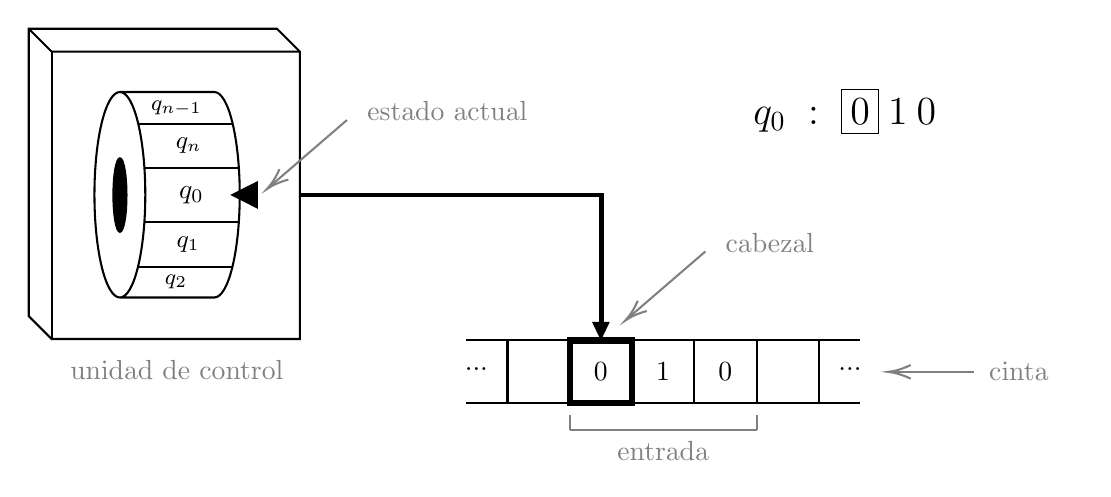
\begin{tikzpicture}[x=0.75pt,y=0.75pt,yscale=-1,xscale=1]
%uncomment if require: \path (0,221); %set diagram left start at 0, and has height of 221

%Flowchart: Direct Access Storage [id:dp5745083904317894] 
\draw   (45.92,32.5) -- (91.42,32.5) .. controls (98.18,32.5) and (103.67,54.66) .. (103.67,82) .. controls (103.67,109.34) and (98.18,131.5) .. (91.42,131.5) -- (45.92,131.5)(33.67,82) .. controls (33.67,54.66) and (39.15,32.5) .. (45.92,32.5) .. controls (52.68,32.5) and (58.17,54.66) .. (58.17,82) .. controls (58.17,109.34) and (52.68,131.5) .. (45.92,131.5) .. controls (39.15,131.5) and (33.67,109.34) .. (33.67,82) ;
%Shape: Cube [id:dp9677041927446011] 
\draw   (132.67,13.07) -- (121.59,2) -- (2,2) -- (2,140.43) -- (13.07,151.5) -- (132.67,151.5) -- cycle ; \draw   (2,2) -- (13.07,13.07) -- (132.67,13.07) ; \draw   (13.07,13.07) -- (13.07,151.5) ;
%Shape: Ellipse [id:dp3944720200277354] 
\draw  [fill={rgb, 255:red, 0; green, 0; blue, 0 }  ,fill opacity=1 ] (42.81,82.14) .. controls (42.81,72.36) and (44.22,64.43) .. (45.95,64.43) .. controls (47.69,64.43) and (49.1,72.36) .. (49.1,82.14) .. controls (49.1,91.93) and (47.69,99.86) .. (45.95,99.86) .. controls (44.22,99.86) and (42.81,91.93) .. (42.81,82.14) -- cycle ;
%Straight Lines [id:da7811026207895715] 
\draw    (57.67,95) -- (103.1,95) ;
%Straight Lines [id:da7715257519556658] 
\draw    (54.52,116.86) -- (99.95,116.86) ;
%Straight Lines [id:da7719478908390764] 
\draw    (55.1,47.86) -- (100.52,47.86) ;
%Straight Lines [id:da44878361199349515] 
\draw    (57.67,69) -- (103.1,69) ;
%Flowchart: Merge [id:dp7750110622325217] 
\draw  [fill={rgb, 255:red, 0; green, 0; blue, 0 }  ,fill opacity=1 ] (111.95,76.14) -- (111.95,88) -- (100.24,82.07) -- cycle ;
%Shape: Rectangle [id:dp3100328904459395] 
\draw   (232.67,152.17) -- (262.67,152.17) -- (262.67,182.17) -- (232.67,182.17) -- cycle ;
%Shape: Rectangle [id:dp1692041741743724] 
\draw  [line width=2.25]  (262.67,152.17) -- (292.67,152.17) -- (292.67,182.17) -- (262.67,182.17) -- cycle ;
%Shape: Rectangle [id:dp5247156403937852] 
\draw   (292.67,152.17) -- (322.67,152.17) -- (322.67,182.17) -- (292.67,182.17) -- cycle ;
%Shape: Rectangle [id:dp1939162798122891] 
\draw   (322.67,152.17) -- (352.67,152.17) -- (352.67,182.17) -- (322.67,182.17) -- cycle ;
%Shape: Rectangle [id:dp955944006123826] 
\draw   (352.67,152.17) -- (382.67,152.17) -- (382.67,182.17) -- (352.67,182.17) -- cycle ;
%Straight Lines [id:da2297213302864911] 
\draw    (382.67,152.17) -- (402.67,152.17) ;
%Straight Lines [id:da0017979141787713981] 
\draw    (382.67,182.17) -- (402.67,182.17) ;
%Straight Lines [id:da5196954519515742] 
\draw    (212.67,182.17) -- (232.67,182.17) ;
%Straight Lines [id:da6250621041798603] 
\draw    (212.67,152.17) -- (232.67,152.17) ;
%Straight Lines [id:da4041928331954272] 
\draw [color={rgb, 255:red, 128; green, 128; blue, 128 }  ,draw opacity=1 ]   (262.67,195.17) -- (352.67,195.17) ;
%Straight Lines [id:da40491651879492707] 
\draw [color={rgb, 255:red, 128; green, 128; blue, 128 }  ,draw opacity=1 ]   (262.67,188.17) -- (262.67,195.17) ;
%Straight Lines [id:da9178129384480556] 
\draw [color={rgb, 255:red, 128; green, 128; blue, 128 }  ,draw opacity=1 ]   (352.67,188.17) -- (352.67,195.17) ;
%Shape: Right Angle [id:dp42415196847546355] 
\draw  [line width=1.5]  (132,82) -- (278,82) -- (278,146) ;
%Straight Lines [id:da05158428581441665] 
\draw    (277.67,128) -- (277.67,149.17) ;
\draw [shift={(277.67,152.17)}, rotate = 270] [fill={rgb, 255:red, 0; green, 0; blue, 0 }  ][line width=0.08]  [draw opacity=0] (8.93,-4.29) -- (0,0) -- (8.93,4.29) -- cycle    ;
%Straight Lines [id:da7132164152395672] 
\draw [color={rgb, 255:red, 128; green, 128; blue, 128 }  ,draw opacity=1 ]   (155.33,46) -- (118.18,78.03) ;
\draw [shift={(116.67,79.33)}, rotate = 319.24] [color={rgb, 255:red, 128; green, 128; blue, 128 }  ,draw opacity=1 ][line width=0.75]    (10.93,-3.29) .. controls (6.95,-1.4) and (3.31,-0.3) .. (0,0) .. controls (3.31,0.3) and (6.95,1.4) .. (10.93,3.29)   ;
%Straight Lines [id:da42945985402945897] 
\draw [color={rgb, 255:red, 128; green, 128; blue, 128 }  ,draw opacity=1 ]   (457.33,167.33) -- (418,167.33) ;
\draw [shift={(416,167.33)}, rotate = 360] [color={rgb, 255:red, 128; green, 128; blue, 128 }  ,draw opacity=1 ][line width=0.75]    (10.93,-3.29) .. controls (6.95,-1.4) and (3.31,-0.3) .. (0,0) .. controls (3.31,0.3) and (6.95,1.4) .. (10.93,3.29)   ;
%Straight Lines [id:da3859416199015755] 
\draw [color={rgb, 255:red, 128; green, 128; blue, 128 }  ,draw opacity=1 ]   (328,109.33) -- (290.85,141.36) ;
\draw [shift={(289.33,142.67)}, rotate = 319.24] [color={rgb, 255:red, 128; green, 128; blue, 128 }  ,draw opacity=1 ][line width=0.75]    (10.93,-3.29) .. controls (6.95,-1.4) and (3.31,-0.3) .. (0,0) .. controls (3.31,0.3) and (6.95,1.4) .. (10.93,3.29)   ;

% Text Node
\draw (73.26,40.18) node  [font=\footnotesize] [align=left] {\begin{minipage}[lt]{24.7pt}\setlength\topsep{0pt}
\begin{center}
$q_{n-1}$
\end{center}

\end{minipage}};
% Text Node
\draw (79.1,58.43) node  [font=\small] [align=left] {\begin{minipage}[lt]{32.64pt}\setlength\topsep{0pt}
\begin{center}
$q_n$
\end{center}

\end{minipage}};
% Text Node
\draw (80.38,82) node  [font=\normalsize] [align=left] {\begin{minipage}[lt]{30.89pt}\setlength\topsep{0pt}
\begin{center}
$q_0$
\end{center}

\end{minipage}};
% Text Node
\draw (78.81,105.93) node  [font=\small] [align=left] {\begin{minipage}[lt]{28.75pt}\setlength\topsep{0pt}
\begin{center}
$q_1$
\end{center}

\end{minipage}};
% Text Node
\draw (72.97,124.18) node  [font=\footnotesize] [align=left] {\begin{minipage}[lt]{25.09pt}\setlength\topsep{0pt}
\begin{center}
$q_2$
\end{center}

\end{minipage}};
% Text Node
\draw (247.67,167.17) node  [font=\normalsize] [align=left] {\begin{minipage}[lt]{20.4pt}\setlength\topsep{0pt}
\begin{center}
\Vtextvisiblespace
\end{center}

\end{minipage}};
% Text Node
\draw (277.67,167.17) node  [font=\normalsize] [align=left] {\begin{minipage}[lt]{20.4pt}\setlength\topsep{0pt}
\begin{center}
$0$
\end{center}

\end{minipage}};
% Text Node
\draw (307.67,167.17) node  [font=\normalsize] [align=left] {\begin{minipage}[lt]{20.4pt}\setlength\topsep{0pt}
\begin{center}
$1$
\end{center}

\end{minipage}};
% Text Node
\draw (337.67,167.17) node  [font=\normalsize] [align=left] {\begin{minipage}[lt]{20.4pt}\setlength\topsep{0pt}
\begin{center}
$0$
\end{center}

\end{minipage}};
% Text Node
\draw (367.67,167.17) node  [font=\normalsize] [align=left] {\begin{minipage}[lt]{20.4pt}\setlength\topsep{0pt}
\begin{center}
\Vtextvisiblespace
\end{center}

\end{minipage}};
% Text Node
\draw (397.67,167.17) node  [font=\normalsize] [align=left] {\begin{minipage}[lt]{20.4pt}\setlength\topsep{0pt}
\begin{center}
$...$
\end{center}

\end{minipage}};
% Text Node
\draw (217.67,167.17) node  [font=\normalsize] [align=left] {\begin{minipage}[lt]{20.4pt}\setlength\topsep{0pt}
\begin{center}
$...$
\end{center}

\end{minipage}};
% Text Node
\draw (307.67,205.17) node  [font=\normalsize,color={rgb, 255:red, 128; green, 128; blue, 128 }  ,opacity=1 ] [align=left] {\begin{minipage}[lt]{61.2pt}\setlength\topsep{0pt}
\begin{center}
entrada
\end{center}

\end{minipage}};
% Text Node
\draw (73.33,166.5) node  [font=\normalsize,color={rgb, 255:red, 128; green, 128; blue, 128 }  ,opacity=1 ] [align=left] {\begin{minipage}[lt]{91.57pt}\setlength\topsep{0pt}
\begin{center}
unidad de control
\end{center}

\end{minipage}};
% Text Node
\draw (214.69,41.83) node  [font=\normalsize,color={rgb, 255:red, 128; green, 128; blue, 128 }  ,opacity=1 ] [align=left] {\begin{minipage}[lt]{74.32pt}\setlength\topsep{0pt}
estado actual
\end{minipage}};
% Text Node
\draw (485.02,167.17) node  [font=\normalsize,color={rgb, 255:red, 128; green, 128; blue, 128 }  ,opacity=1 ] [align=left] {\begin{minipage}[lt]{30.35pt}\setlength\topsep{0pt}
cinta
\end{minipage}};
% Text Node
\draw (387.35,105.17) node  [font=\normalsize,color={rgb, 255:red, 128; green, 128; blue, 128 }  ,opacity=1 ] [align=left] {\begin{minipage}[lt]{74.32pt}\setlength\topsep{0pt}
cabezal
\end{minipage}};


\draw (400.69,41.83) node  [font=\normalsize,color={rgb, 255:red, 0; green, 0; blue, 0 }  ,opacity=1 ] [align=left] {\begin{minipage}[lt]{74.32pt}\setlength\topsep{0pt}
\Large{$q_0\;:\;\fbox{$0$}\:1\:0$}
\end{minipage}};

\end{tikzpicture}